\documentclass[a4paper,11pt]{article}

\usepackage[T1]{fontenc}
\usepackage[utf8]{inputenc}
\usepackage{graphicx}
\usepackage{xcolor}

\renewcommand\familydefault{\sfdefault}
\usepackage[defaultmono]{droidmono}

\usepackage{enumerate}
\usepackage{hyperref} 

\usepackage{geometry}
\geometry{total={210mm,297mm},
left=25mm,right=25mm,%
bindingoffset=0mm, top=20mm,bottom=20mm}


\linespread{1.3}

\newcommand{\linia}{\rule{\linewidth}{0.5pt}}
\renewcommand{\arraystretch}{1.5}
\makeatletter
\renewcommand{\maketitle}{
\begin{center}
\vspace{2ex}
{\huge \textsc{\@title}}
\vspace{1ex}
\\
\linia\\
\@author \hfill \@date
\vspace{4ex}
\end{center}
}
\makeatother

\usepackage{fancyhdr}
\pagestyle{fancy}
\lhead{}
\chead{}
\rhead{}
\lfoot{ChallP FS16}
\cfoot{}
\rfoot{Page \thepage}
\renewcommand{\headrulewidth}{0pt}
\renewcommand{\footrulewidth}{0pt}
%

\begin{document}

\title{Z-Wave Factsheet}

\author{fbinna, vmeier, laquino}

\date{2016}

\maketitle

\section*{Generell}
\begin{tabular}{| p{3.5cm} | p{10cm} |}
	\hline
	\textbf{Einsatzgebiet} & Home-Automation \\\hline
	\textbf{Topologie} & Mesh \\\hline
	\textbf{Range} & bis zu 100m zwischen 2 Nodes \\\hline
	\textbf{Maximaler Range} & Durchschnittlich 200m (Weiterleitung über 4 Hops) \\\hline
	\textbf{Anzahl Geräte pro Netzwerk} & 232 \\\hline
	
\end{tabular}

\subsection*{Gerätetypen}
\begin{itemize}
 \item Elektrische Schalter (ergänzend oder Ersatz für physischen Schalter)
 \item Elektrische Dimmer (ergänzend oder Ersatz für physischen Schalter)
 \item Motoren (zum Öffnen / Schliessen von Fenstern, Rollläden etc.)
 \item Bildschirme, LED-Displays, Sirenen etc. (Signal-Quellen)
 \item Sensoren (Themometer, Hygrometer etc.)
 \item Thermostat Controller (Thermostat Radiator Valves, Bodenheizung-Controller etc.)
 \item Fernbedienungen (Universelle Infrarot-Fernbedienungen, spezielle Z-Wave Fernbedienungen ...)
 \item USB Sticks und IP Gateways (für Fernsteuerung über PC / über Internet)
\end{itemize}

\subsection*{Netzwerk-Informationen}
Ein Netzwerk besteht jeweils aus einem (oder in Spezialfällen aus mehreren) Controller und mehreren Slaves. Die Komponenten können über eine HomeID und NodeID eindeutig identifiziert werden.\\\\
\begin{tabular}{| p{3.5cm} | p{10cm} |}
	\hline
	\textbf{HomeID} & 32bit; Hersteller weist dem Controller eine ID zu, der die HomeID des Netzwerks bestimmt\\\hline
	\textbf{NodeID} & 8bit; Controller weist allen Slaves eine NodeID zu\\\hline
\end{tabular}~\newpage

\section*{Protokoll-Spezifikationen}
\begin{figure}[h!t]
	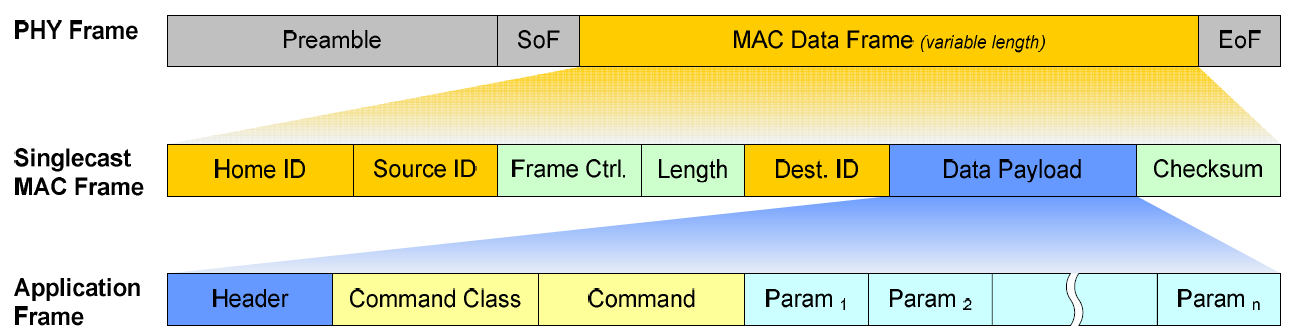
\includegraphics[width=\textwidth]{images/frame.png}
\end{figure}

\subsection*{Physical Layer}
\begin{tabular}{| p{3.5cm} | p{10cm} |}
	\hline
	\textbf{Datenübertragungs-rate} & 9.6kbps / 40kbps / 100kbps\\\hline
	\textbf{Frequenz} &  {\textbf{Europa}: 868.42 MHz (SRD); \textbf{USA}: 908.42 MHz (ISM)} \\\hline
	\textbf{Encoding} & Machester (9.6kbps) / NRZ (40kbps / 100kbps) \\\hline
	\textbf{Maximaler Range} & Durchschnittlich 200m (Weiterleitung über 4 Hops) \\\hline
	\textbf{Anzahl Geräte pro Netzwerk} & 232 \\\hline
\end{tabular}

\subsection*{Application Layer}
\subsubsection*{Command classes}
Z-Wave kommuniziert den Geräten, unabhängig von deren Funktionalität, Kommandos über 3 verschiedene ``Command classes``. Die Interpretation des übertragenen Kommandos ist dann den Geräten überlassen.\\\\
\begin{tabular}{| c | c | p{6cm} |}
	\hline
	\textbf{Name} & \textbf{Wertrange}& \textbf{Funktion}\\\hline
	SET & 0 - 255 & Setzen eines Wertes \\\hline
	GET & - & Anfrage des aktuell eingestellten Wertes \\\hline
	REPORT & 0-255 & Response mit aktuellem Wert auf GET-Request\\\hline
\end{tabular}
~
\newpage

\subsection*{Security}
\begin{tabular}{| p{3.5cm} | p{10cm} |}
	\hline
	\textbf{Preshared Key} & 128bit Network Key; Von Controller generiert\\\hline
	\textbf{Cipher \& MAC-Keys} & 128bit; Von Netzwerk Key abgeleitet\\\hline
	\textbf{Nonce} & 64bit; Gegen Replay-Attacken\\\hline
	\textbf{Encryption} & AES-OFB\\\hline
	\textbf{Data-Authentication} & AES-CBCMAC\\\hline
\end{tabular}

\section*{Eignung im Bereich IoT}
\subsection*{Energieverbrauch}
Die Z-Wave Technologie versucht den Energieverbrauch möglichst gering zu halten. Das wird erreicht, indem die Z-Wave Units im power-safe Modus arbeiten und so nur 0.1\% aktiv sind. Durch den geringen Energieverbrauch können die Z-Wave Units in batteriebetriebenen Geräten (z.B. Fernbedienungen, Rauchmelder und Sensoren) verbaut werden.

\subsection*{Eignungsbereiche}
\subsubsection*{SmartHome}
Z-Wave arbeitet im sub-gigahertz Bereich, und vermeidet so die Überlagerung mit Wifi- und Bluetoothtechnologien. Bei der Entwicklung wurde speziell beachtet, dass die Reichweite, durch Wände und andere Hindernisse nicht zu stark beeinträchtigt wird.

\subsubsection*{Outdoor}
Z-Wave wurde ursprünglich für den Gebrauch in Gebäuden entwickelt. Es ist aber prinzipiell Möglich auch Systeme im Freien zu entwickeln. Die Reichweite beträgt ungefähr 100m (Die SAW filter des Herstellers Sigma Design begrenzen die Richweite auf 30m), das heisst es ist mit Hilfe eines Netzes möglich grössere Flächen abzudecken.

\subsection*{Entwicklung}
Für die Entwicklung ist kein teures SDK nötig. Es gibt eine freie API (open-zwave), die es ermöglicht auf verschiedensten Systemen Z-Wave Technologie einzusetzen. Zudem ist ein Raspberry PI "daughter board" verfügbar, die den Einsatz solcher Chips nochmals vereinfacht.

\section*{Quellen}

\href{http://www.z-wave.com/faq}{Offizielles Z-Wave FAQ}\\
\href{https://www.youtube.com/watch?v=KYaEQhvodc8}{BlackHat 2013 - Hacking Z-Wave}\\
\href{http://wiki.zwaveeurope.com/index.php?title=Z-Wave_Technical_Handbook}{Z-Wave Europe Wiki - Handbook (Linksammlung)}\\
\href{http://wiki.zwaveeurope.com/index.php?title=Z-Wave_Application_Layer}{Z-Wave Europe Wiki - Application Layer Details}\\
\href{https://en.wikipedia.org/wiki/Z-Wave}{Wikipedia - Z-Wave}
\href{https://www.sensepost.com/cms/resources/conferences/2013/bh_zwave/Security\%20Evaluation\%20of\%20Z-Wave_WP.pdf}{Z-Wave Security Evaluation}


\end{document}
